\chapter{Performance Comparison and Evaluation}
In this chapter, we describe our experiments regarding two research questions we proposed in Chapter 1. The experiments based on the DevOps toolchains we implemented in Chapter 4.
\par
In Section 5.1, we will examine how does the serverless compute engine for containers (Amazon ECS on AWS Fargate) could influence the performance of non-integrated toolchains. Thus, in the experiment, we implement the solution with a different type of cloud environment (with/without serverless) as a comparison group.
In Section 5.2, we focus on answering research question 2, in which we will compare the performance of continuous delivery pipeline composed of fully-managed serverless DevOps tools in AWS with our Jenkins-based pipeline that runs on the virtual machine.
\section{Experiment 1: Experiment on Serverless Container Services}
The Docker agent has already been supported by many CI/CD tools ad we introduced in Chapter 4.
The serverless container services in AWS (AWS Fargate) provides the possibility to ease the infrastructure management task for the Docker build agents.
This experiment is a controlled experiment which examines whether serverless container service could improve the continuous delivery pipeline from various perspectives.
\subsection{Test Task and System Description}
In this experiment, we run the continuous delivery process of a Spring Boot web application with our DevOps toolchain. From the experiments, we could verify our assumption in Chapter 3 and better-answering RQ 1.
\par
As we described in Chapter 4, the continuous delivery pipeline includes the following steps:
\begin{enumerate}
\item \textit{Checkout}: Pull the most recent change from GitHub repository
\item \textit{Build}: Build the application with Gradle, with automating testing with JUnit integrated into Gradle.
\item \textit{Build the docker image}: Build the docker image of our Spring Boot application.
\item \textit{Push to Container Registry}: Push the docker image from the last step to the AWS elastic cloud registry (ECR) for further deployment.
\end{enumerate}
\par
In these four steps, the step "Build", and "Checkout" is being done in parallel within the ECS cluster. As we mentioned in CH4, when the new job started in the Jenkins master server, Jenkins will provision a new container instance within the ECS cluster. The container is managed directly by AWS, so we don't need to create and manage the virtual machine that runs the container. We use this setup in our initial implementation as the control group.
\par
In the experimental group, we replace AWS Fargate with traditional VM, which is EC2 in the Amazon Web Services.The parallelisation pattern remains the same; this means as in the control group, only the first two steps are being run distributively in the Jenkins nodes. The EC2 instances belong to an auto-scaling group that will scale up when CPU Utilisation rate reach 70\%. The initial size for an auto-scaling group is one EC2 virtual machine.
\par
Figure \ref{fig:ex1} shows the architecture of two groups in this experiment. The experimental group on the left is a Jenkins server with the traditional virtual machine as workers node that hosting the container agent. The architecture of the control group on the right has agent nodes dynamically provisioned as serverless containers hosed by AWS Fargate.
\begin{figure}[h]
\centering
\begin{minipage}{0.45\textwidth}
\centering
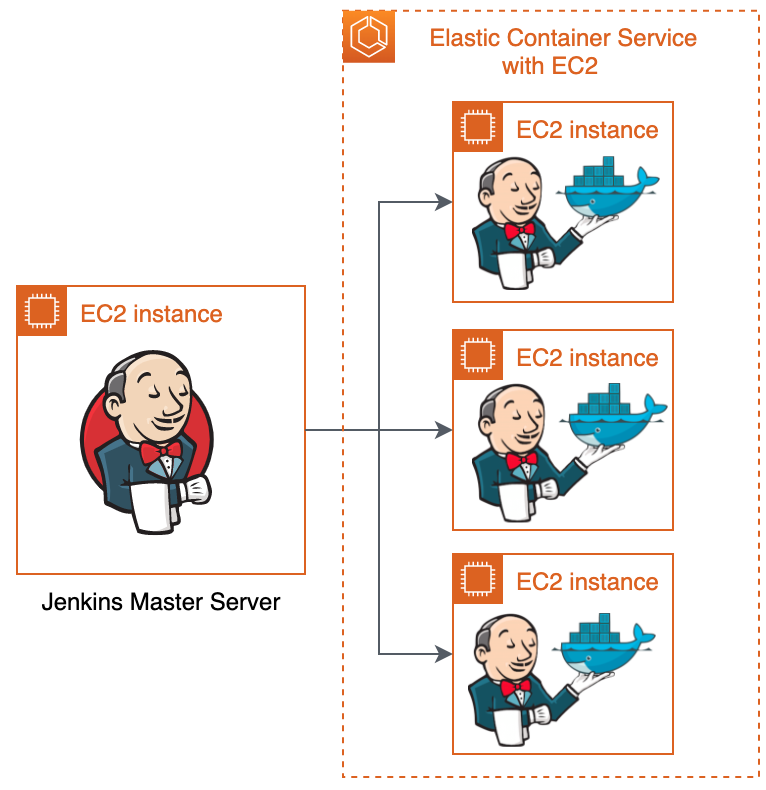
\includegraphics[width=\textwidth]{pics/jenkins-on-vm.png} % first figure itself
\end{minipage}\hfill
\begin{minipage}{0.54\textwidth}
\centering
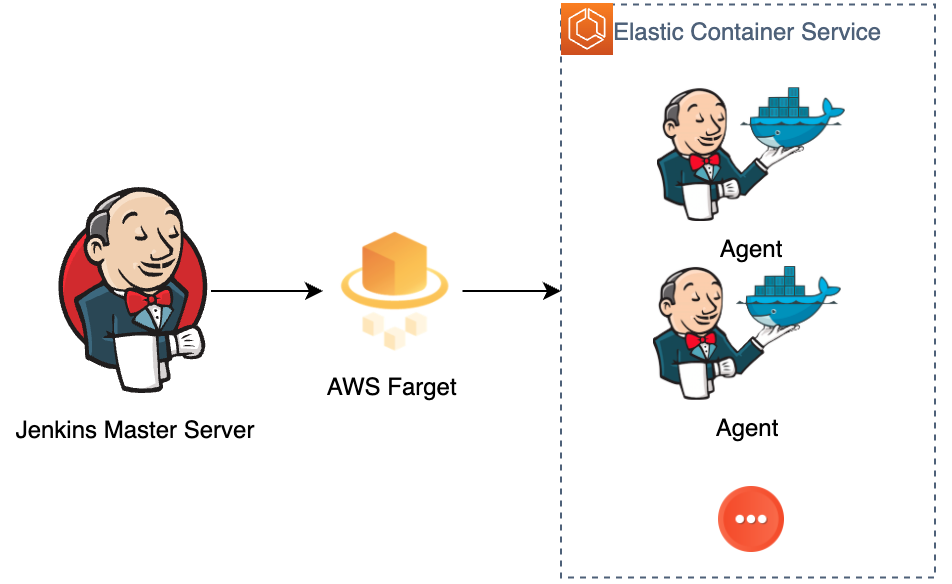
\includegraphics[width=\textwidth]{pics/jenkins-on-fargate.png} % second figure itself
\end{minipage}
\caption{Architecture diagram of the test Jenkins cluster with agents running in traditional virtual machines (left) and on ECS with AWS Fargate (right)}
\label{fig:ex1}
\end{figure}
\subsubsection{Hardware}
The hardware of the instance that runs Jenkins agents is the independent variable that exposed to the change in the experiment.
\par
The experiments are conducted on Amazon Web Services (AWS). The hardware of Jenkins master node in both experiment groups is the same, which is EC2 instance of type t3.medium with two virtual CPU, 4 GB RAM and 30 GB disk. The EC2 instances as worker node are type t3.small, with two virtual CPU and 2GB RAM. Each EC2 instance can run one container at the same time.
\par
In the control group, which is the implementation we presented in CH4, the Jenkins agents run on AWS ECS powered by AWS Fargate. The virtual hardware resources that are allocated to each serverless container is two virtual CPU, and 2 GB of RAM. The identical hardware setup between to groups makes sure that each container shares the same hardware resources as in another group, so the hardware will not affect the result.
\subsubsection{Software}
We maintain the same software setup in each group. The versions of the software are all in the latest version as for February 2020. The operating System of EC2 instance that runs Jenkins master node is Ubuntu Server 18.04. The version of Jenkins that runs on the server is 2.222.3. For connect ECS and Fargate which works as the Jenkins agents, we use Jenkins plugin "Amazon Elastic Container Service (ECS) / Fargate", version 1.34. The container in Fargate/EC2 for running the Checkout and Build steps is from our developed docker image, which can be seen at \footnote{https://hub.docker.com/r/dry1995/jnlp}. The docker image includes essential dependencies that will be used to build the Spring Boot application. It's the base image include a program which allows container connects Jenkins master as an agent. The "Build" step in our pipeline uses Gradle (version: 6.2.1) as the build tool for the application,
with OpenJDK 1.8.0.252 as Java virtual machine (JVM).
This step also includes the automated testing and code analysis, as plugins of Gradle. 
\par
To shows how does the two setups performance within the teams with different sizes, we run by run the different number of tasks parallel through the pipeline. This scenario simulates the different team size and shows the scalability when it comes to the need for task parallelisation in larger organisations. It also imitates the DevOps process of a microservices software project, which could have multiple jobs for different service runs in parallel.
\subsection{Performance Properties and Evaluation}
We run the pipeline through 2 different setups, and we will get the result of the following properties:
\begin{itemize}
\item \textit{Runtime} describes the total time for finishing all the jobs. If the jobs run in parallel, the runtime is from the start of jobs until the end of the last finished job.
\item \textit{Cost Structure} describes the daily cost of 2 setups under the same workload, within the same period.
\item \textit{Resource Utilisation} describes the average CPU/RAM usage for each instance during a single run of the pipeline. The purpose of this comparison is to show the performance of the same application in a different environment (EC2 and Fargate).
\end{itemize}
\subsection{Result and Evaluation}
Here shows the result of this experiment. We also evaluate our experiment result by analysing the factors that lead to the results.
\subsubsection{Runtime}
We first compare the runtime of these two setups. Except for test the runtime of single job runs with two setups respectively, we also test the runtime of each pipeline setup under different number jobs executed in parallel. Figure \ref{fig:runtime} shows the test result.
\begin{figure}[h]
\centering
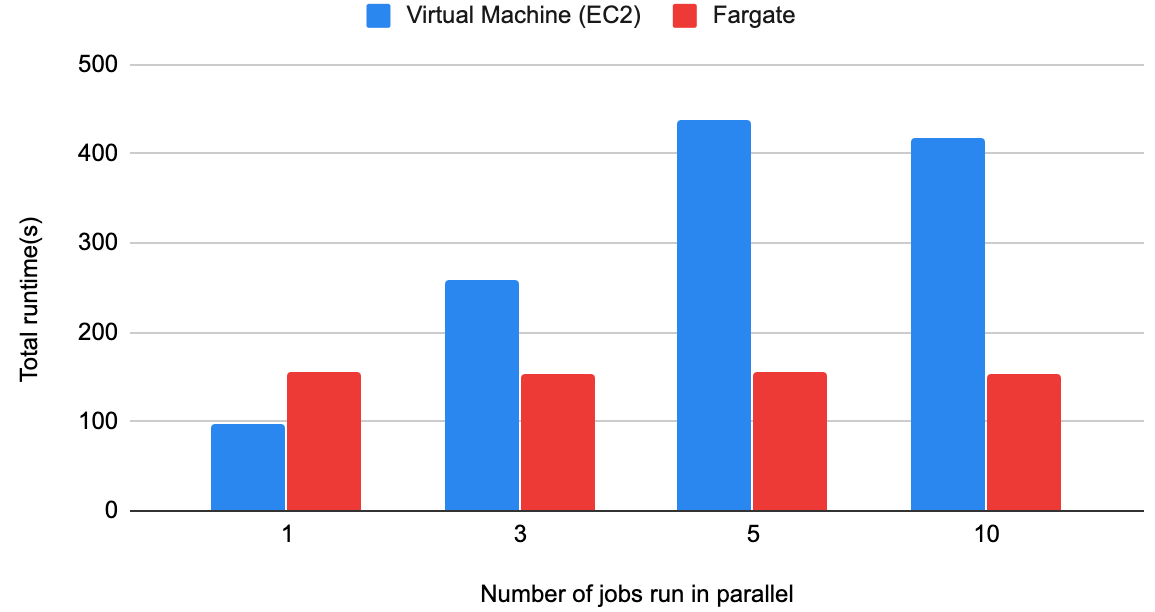
\includegraphics[width=0.99\textwidth]{pics/runtime.png}
\caption{Runtime of Pipeline with Different Jenkins Agents Under Different Number of Jobs Runs in Parallel}
\label{fig:runtime}
\end{figure}
\par
The test result shows that when it comes to the execution of a single task. The traditional VM has a faster delivery speed over serverless solution (AWS Fargate). However, with the number of jobs that run in parallel increases, the total runtime on the traditional VM decrease. On the contract, on the serverless solution(Fargate), the runtime remains almost the same.
\par
We analyse the reason behind this result, and we found out that the longer runtime with the single job on Fargate is because the longer starting time of Jenkins agent. In EC2, the Jenkins will simply provision a Docker container within EC2 VM, and connect to the Jenkins master node. However, in Fargate, the Jenkins can only connect to the agent once AWS finishes the initialisation of underlay infrastructure that runs the serverless container, which takes a significantly longer time. The slow provisioning shows one of the limitations of serverless computing (cold-start) that we mentioned in Section \ref{servlesslimitation}.
\begin{figure}[!h]
  \centering
  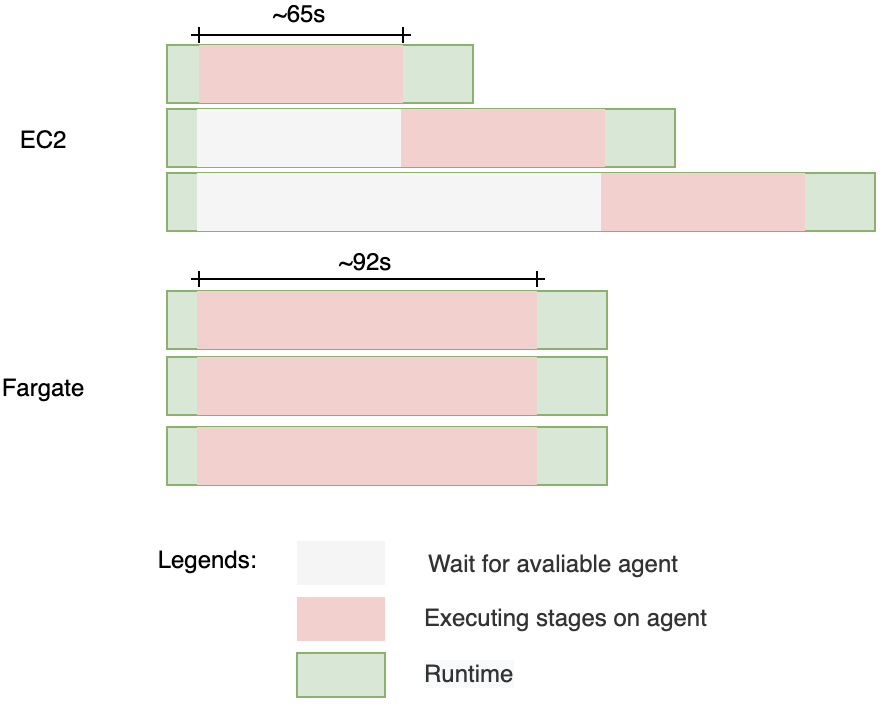
\includegraphics[width=0.90\textwidth]{pics/parallel.png}
  \caption{Execution Mode of Pipelines with Different Jenkins Agents}
  \label{fig:parallel}
  \end{figure}
\par
When it comes to parallel job execution, the performance of Fargate is significantly better. The performance difference is because, in Fargate, each container runs on an independent instance on AWS's infrastructure. Therefore, AWS provisions one Fargate instance for each running job. The independence between Fargate instance ensures the agent will not compete for the resource. On the other hand, when we run multiple agents in our EC2 instance, due to the limitation of resource, part of running jobs has to wait until the resource on EC2 instance available until they can start the execution. To further investigate the reason for the result, we observe the parallel execution mode when it runs three jobs in parallel. Figure \ref{fig:parallel} shows the execution modes. We find that the easily scalable character (mentioned in \ref{servlesslimitation}) helps the serverless suites better with the parallel task. The long wait time is the reason that makes the total runtime in EC2 much longer.
\par
We also notice that in Figure 5.2, when the parallel task reaches 10, the EC2 runtime becomes shorter. The shorter runtime of EC2 is because we set auto-scaling for our EC2 instance. So in the later part of our experiment, the EC2 scaled from 1 to 2 and then to 3. Nevertheless, even with 3 EC2 instances, only three jobs are allowed to run in parallel, while in Fargate is easy to have ten jobs runs in the complete parallel method. This because the scaling of EC2 VMs is much slower because it is heavier to create a VM than create a new Fargate instance. The other reason is the auto-scaling of EC2 VM is triggered by reaching certain resource utilisation threshold, but in Fargate is based on task number(Jenkins agent number). Even we set the scaling policy of EC2 to a more aggressive pattern, the AWS still more "hesitate" to create new instances compared within the Fargate. 
Therefore, in the real-life software development, when the number of jobs surges in Jenkins cluster, the Fargate could react faster in terms of scaling. And when the job drops, Fargate also scale-in faster, which saves cost.
\subsubsection{Resource Utilization}
We compared the average resource utilisation within containers that runs Jenkins agent in two setups. The data from the AWS CloudWatch (Figure \ref{fig:utilizationecs}) shows that the resource utilisation rate is similar in these two setups. The similarity is because the "run in the same way regardless of the host environment" \cite{WhatisaC60:online} feature of Docker container that we mentioned in Section \ref{docker}.
\begin{figure}[h]
\centering
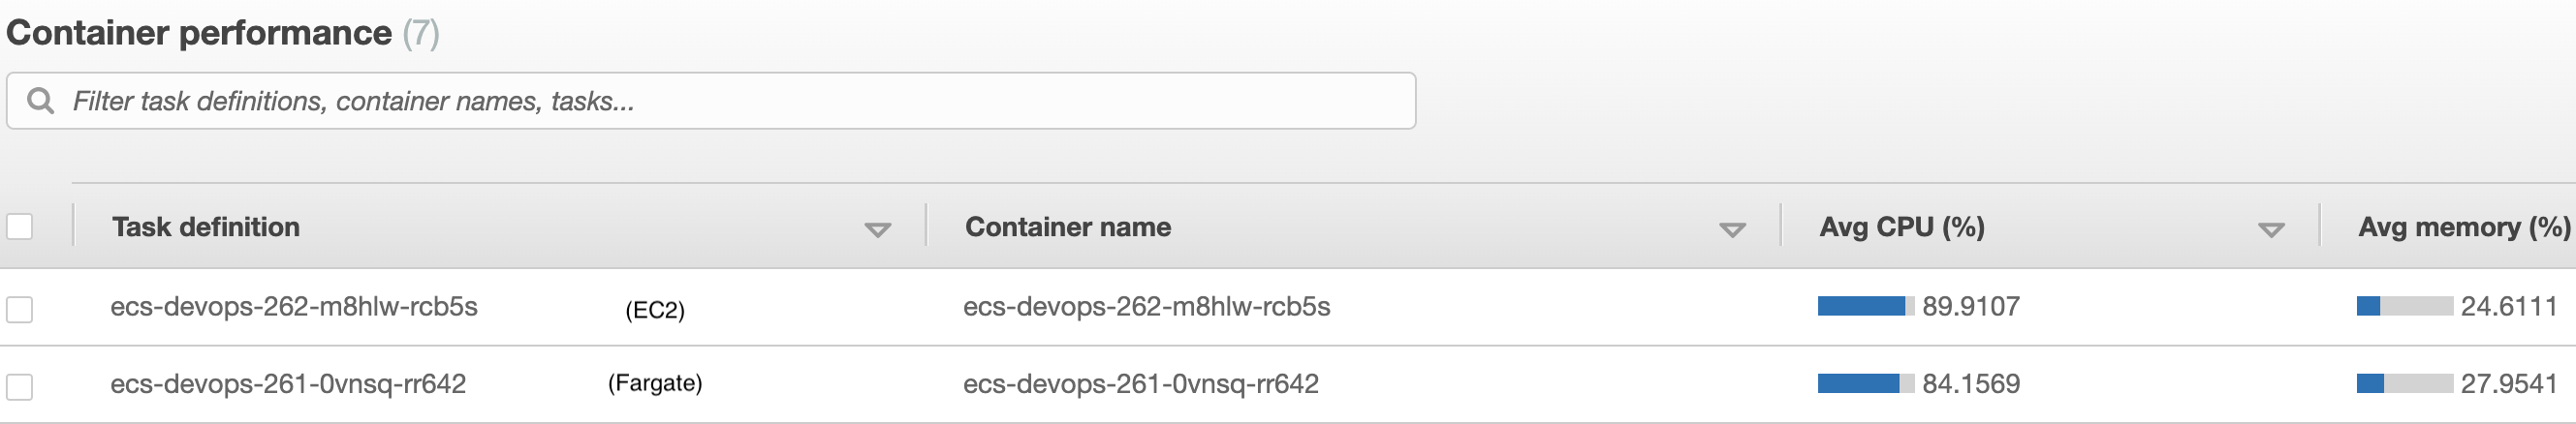
\includegraphics[width=0.99\textwidth]{pics/utilizationecs.png}
\caption{The comparison of Resource Utilization}
\label{fig:utilizationecs}
\end{figure}
\subsubsection{Cost Analysis}
The container orchestration service ECS itself is free of charge. We only pay for the resources we are using, which is Fargate or EC2 virtual machine.
\par
In AWS Fargate we pay only by resource we are using and the runtime. The price for Fargate service in EU(Stockholm) is \$0.04165 per GB RAM per hour plus \$0.0049 per vCPU per hour \footnote{https://aws.amazon.com/fargate/pricing/}. Thus, in our experiment setup (2vCPU, 2 GB RAM), the price should be \$0.0931 per running agent for one hour's runtime.
In AWS EC2 our cost depends on the type of VM we are using. The type of VM we use for running Jenkins agents is t3.small that costs \$0.0216 per hour \footnote{https://aws.amazon.com/ec2/pricing/on-demand/}. The Fargate-based Jenkins agent is more expensive than EC2-based agent.
\par
However, the pay-per-use characteristic of serverless service makes Fargate more competitive in terms of cost. The instance only up and run when Jenkins master distributes the job. Once the job finished, the AWS will terminate Fargate instance immediately when it finds no container is running on it. However, EC2 not so flexible due to the resource-utilisation-based scaling policy. The EC2 instance is not scaled in immediately after job finished, and the user has to pay for the instance runtime before it gets terminated -- even there is no job running in EC2 instance any more. So depends on the frequency and length of the build task, the user could have runtime per hour when using Fargate instance.
\subsection{Conclusion}
In this experiment, we compare the serverless (AWS Fargate) and non-serverless solution (EC2) for hosting distributed continuous delivery pipeline. The experiment shows that the performance of the serverless solution is worse when it comes to single job execution, which is because of the cold-start issue with serverless computing. However, in terms of the parallel job executing, the serverless solution has better performance over traditional VM. 
\begin{table}[h!]
  \begin{center}
      \begin{tabular}{|l|l|l|}
      \hline
       &
        EC2 Agents &
        Fargate Agents \\ \hline
      Build Time &
        \begin{tabular}[c]{@{}l@{}}98s for a single task.\\ Largely increases when\\ run multiple tasks in \\ parallel\end{tabular} &
        \begin{tabular}[c]{@{}l@{}}155s for a single task.\\ Remains unchanged when\\ multiple task runs in \\ parallel\end{tabular} \\ \hline
      Cost &
        \begin{tabular}[c]{@{}l@{}}Lower per hour price\\ (\$0.0216)\end{tabular} &
        \begin{tabular}[c]{@{}l@{}}Higher per hour price\\ (\$0.0931), however the\\ billable hour is shorter,\\ the total price could be\\ lower.\end{tabular} \\ \hline
      \end{tabular}
      \caption{Conclusion of Experiment 1}
      \label{tab:exp1}
  \end{center}
      \end{table}
\par
\label{micros}
An better parallel execution performance is meaningful for apply DevOps practice in the microservices development. A microservices could have hundred of services. In the philosophy of microservices, the release of each service should be independently \cite{dehghani2018break}. To ensure this, one practices it to use one pipeline for each service. However managing a hundred pipelines is not an easy task, and better practice is to have multiple services share a single pipeline \cite{HowtoSca9:online}. Therefore, when multiple services share the same pipeline, this improvement allows services to be released independently without waiting for each other.
\par
In term of cost, the serverless solution is more expensive per hour. However, the difference could be offset by the less runtime. Moreover, resource utilisation is similar in both solutions. Table \ref{tab:exp1} show a comparison between two experimental groups.
\section{Experiment 2: Experiment on Integrated DevOps Toolchain}
For solving the RQ2, we compare the implementation of our design of two different the DevOps toolchain -- the non-integrated Jenkins based toolchain and the AWS DevOps toolchain implementation with AWS DevOps tooling.
\subsection{Test Task and System Description}
This second experiment is similar to the first experiment, and we deliver our case project through two DevOps toolchains. The first toolchain is our Jenkins-based toolchain in Section 4.2, with agents runs on AWS Fargate. The second toolchain is the toolchain with AWS DevOps tooling that we described in Section 4.3.
\par
During the experiment, we have set up as follows:
\paragraph{Hardware}
AWS DevOps tools allow us to select the hardware configuration for underlying computing resources. The configuration we chose is two virtual CPU and 3 GB RAM.
The Hardware configuration for Jenkins build agent is two virtual CPU and 4 GB RAM. We cannot set the RAM to 3 GB since AWS Fargate is not allowing \footnote{https://docs.aws.amazon.com/AmazonECS/latest/developerguide/task-cpu-memory-error.html} RAM to below 4GM when using two virtual CPU. However, we still allowed to set an additional software RAM limit to the build agent runs in Fargate agent. Thus, we limit the RAM that a running build agent to 3 GB, which ensure both setups have identical hardware configuration.
\paragraph{Software}
The version of Jenkins that runs on the server is 2.222.3. We use Jenkins plugin" Amazon Elastic Container Service (ECS) / Fargate", version 1.34 for connecting ECS and Fargate which works as the Jenkins agents. The Jenkins cluster has the same configuration as the last experiment. The built environment in both setups is the same, with Gradle (version:6.2.1) and JVM version is OpenJDK 1.8.0.252.
\subsection{Performance Properties and Evaluation Criteria}
We run the pipeline on these two different setups, and we will get the result of the following properties:
\begin{itemize}
\item \textit{Runtime} describes the total time for finishing all the jobs. If the jobs run in parallel, the runtime is from the start of jobs until the end of the last finished job. AWS monitors it's parallel execution ability in the document\footnote{https://aws.amazon.com/codepipeline/features/}\footnote{https://aws.amazon.com/codebuild/features/} of both CodePipeline and CodeBuild, thus we will also validate this ability by analysing the parallel executing pattern of AWS integrated toolchain. \label{aws_parallel}
\item \textit{Cost Structure} describes the daily cost of two setups under the same workload, within the same period.
\end{itemize}
The resource utilisation comparison is not available in the experiment since we cannot get the resources utilisation in underlying hardware resource when running AWS DevOps tools.
\subsection{Quantitative Experiment Result and Evaluation}
This section shows the result of our experiment. We also give an evaluation and analysis of the reason behind the result.
\subsubsection{Runtime}
As in Experiment 1, we compared the running time of each toolchain under different loads \footnote{Workload refers to the different number of jobs running in parallel in the two pipelines}. We only compare the runtime without the final deploy stage. This is because, first, although we can still use the AWS toolchain to deploy to ECS in the same way as the non-integrated toolchain: by using the AWS CLI in CodeBuild to deploy. However, by doing so, we skipped CodeDeploy and instead deployed our project using CodeBuild. This is not a natural practice in production because there is another tool dedicated to deployment (CodeDeploy). Secondly, the deployment mode used in CodeDeploy is very different in terms of the speed of the deployment method used in Jenkins. 
\begin{figure}[!h]
  \centering
  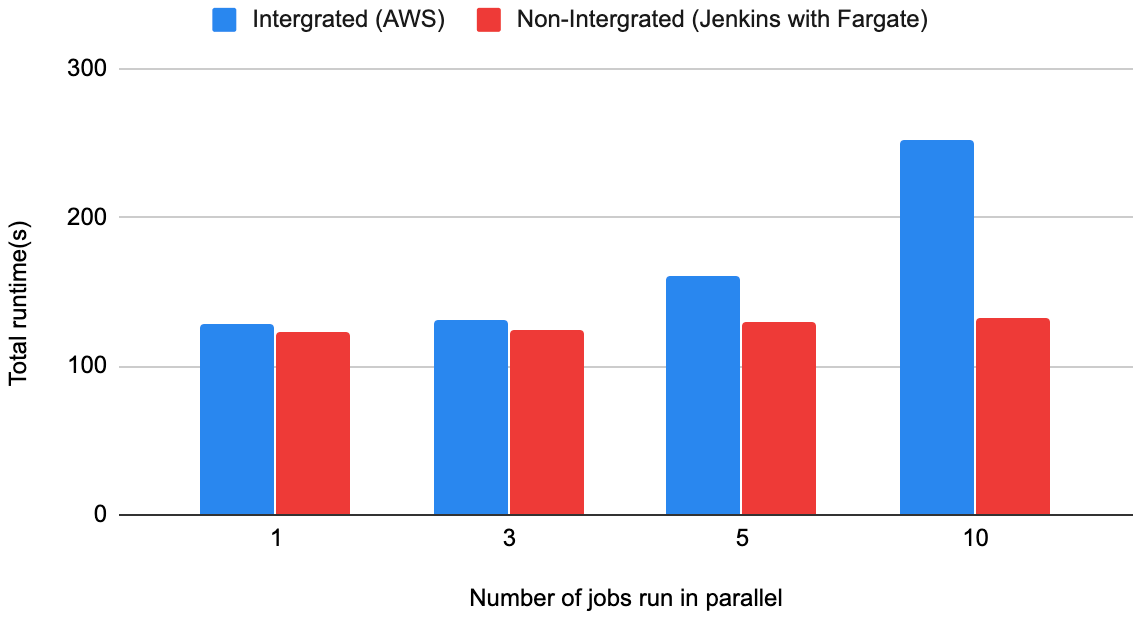
\includegraphics[width=0.80\textwidth]{pics/compare-aws.png}
  \caption{Runtime of the pipeline with on Different Toolchain}
  \label{fig:compareaws}
\end{figure}
Figure \ref{fig:compareaws} shows the result of this experiment. The runtime of integrated toolchain increases with the number of the task runs in parallel, while the non-integrated toolchain remains stable regardless of the number of parallel tasks. We will analyse the reason later in this section.
\par
From Figure \ref{fig:stage_runtime}, we can see that during the execution of a single job, tow toolchains have similar runtime. The similar runtime is because the build stage which takes most of the runtime, is running in a similar environment in both toolchains. Both execution environment is within a Docker container runs with the same hardware in AWS. Although, the Docker image for the container is different in two toolchains, and we are not sure what if the actual hardware is the same since we have no visibility to the hardware in both toolchains. However, still, the performance is not so different in both toolchains.
\par
We further observe the time allocation between stages within the runtime in both toolchains. The figure shows our observation. To get the runtime in Figure \ref{fig:stage_runtime}, we run the pipeline in each toolchain for five times and get the average runtime of each stage. The first difference shows in Figure \ref{fig:stage_runtime} is that the Git Checkout stage in AWS integrated toolchain does not run on the container build agent. Instead, it is running in the unknown environment fully managed by AWS.
\begin{figure}[!h]
  \centering
  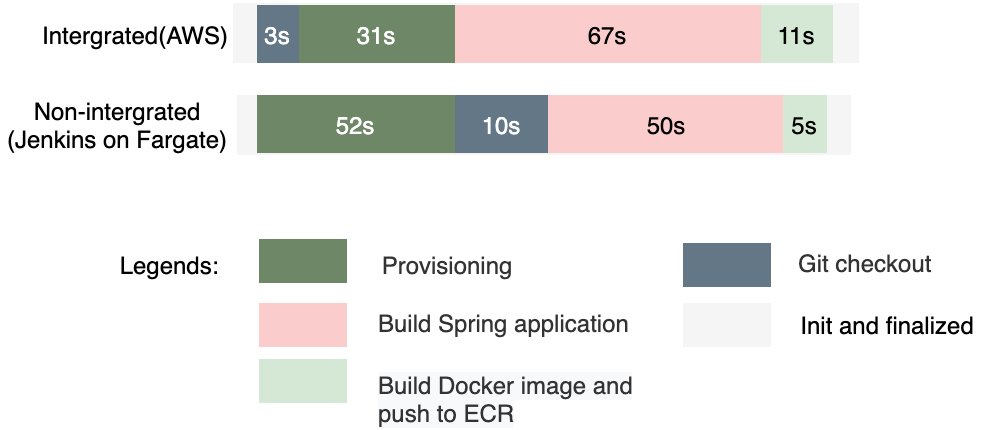
\includegraphics[width=0.99\textwidth]{pics/stages.png}
  \caption{Observation of Runtime of Each Stage on Two Toolchains}
  \label{fig:stage_runtime}
  \end{figure}
\par
We also compared used GitHub and use CodeCommit for the source control in the AWS integrated toolchain. 
We observed that it takes 10 seconds to do the git checkout when using third-party tools (GitHub) as the source control system. During these 10 seconds, the actual Git checkout only takes around 5 seconds, while the AWS toolchain does not do anything in the first 5 seconds. We presume that AWS provisions environment for runs the Git checkout stage in this 5 second, so this stage is also running in a serverless environment within AWS. However, we are not allowed to configure anything in this environment. In contract, it only takes 3 seconds to check out new code from CodeCommit and no waiting time before the checkout. This speed difference could because of the CodeCommit is the part of the AWS services. Thus it has faster data transfer between CodePipeline, or because of no environment provision needed before checkout.
\par
 The second difference is that in AWS integrated toolchain, the provisioning of the build environment is much faster. We presume this is due to AWS manages both build agent and this toolchain, and AWS is optimising the provisioning process of the build environment. Furthermore, the cloud instance that runs build environment in CodeBuild might already be started (used for the build task of other users) before CodePipeline sends our build job to CodeBuild. On the other hand, instances (Fargate) that run Jenkins agents is a cold start, which means it is not running before we send build job there.
 Nevertheless, we can also notice that the build time in the AWS integrated toolchain takes a longer time. It is hard for us to find the reason since the hardware configuration used by AWS is unknown except the size of RAM and the number of virtual CPU.
\par
 Also, we observe that with the workload goes up, the runtime of AWS integrated toolchain increases with it. We already answered why the runtime of the pipeline in our non-integrated toolchain with agent runs in AWS Fargate does not change over time in Section 5.1.3. To explain this, we also check the runtime of each stage when runs several jobs in parallel. We notice that when it has multiple jobs runs in parallel, essential if the parallel jobs' number goes over five. AWS will start limiting the resource allocation, which limits the number of jobs that runs at the same time. As a result, part of our running jobs has to enter the "Queued" status before entering the "Provisioning" stage. In then jobs we run in parallel for the experiment, the time spent for queuing for resource various from 1 second (get resource allocated directly) to 130 seconds. Among these ten jobs, four jobs were put into the queue before resource are available to them. Figure \ref{fig:queued} shows the distribution of queued time among jobs. This validates the claim\footnote{https://aws.amazon.com/codepipeline/features/} from AWS about parallel execution ability, which we mentioned in Section \ref{aws_parallel}. However, the parallel pipeline execution is not fully in parallel but with some limitations on available resources.
 \begin{figure}[!h]
  \centering
  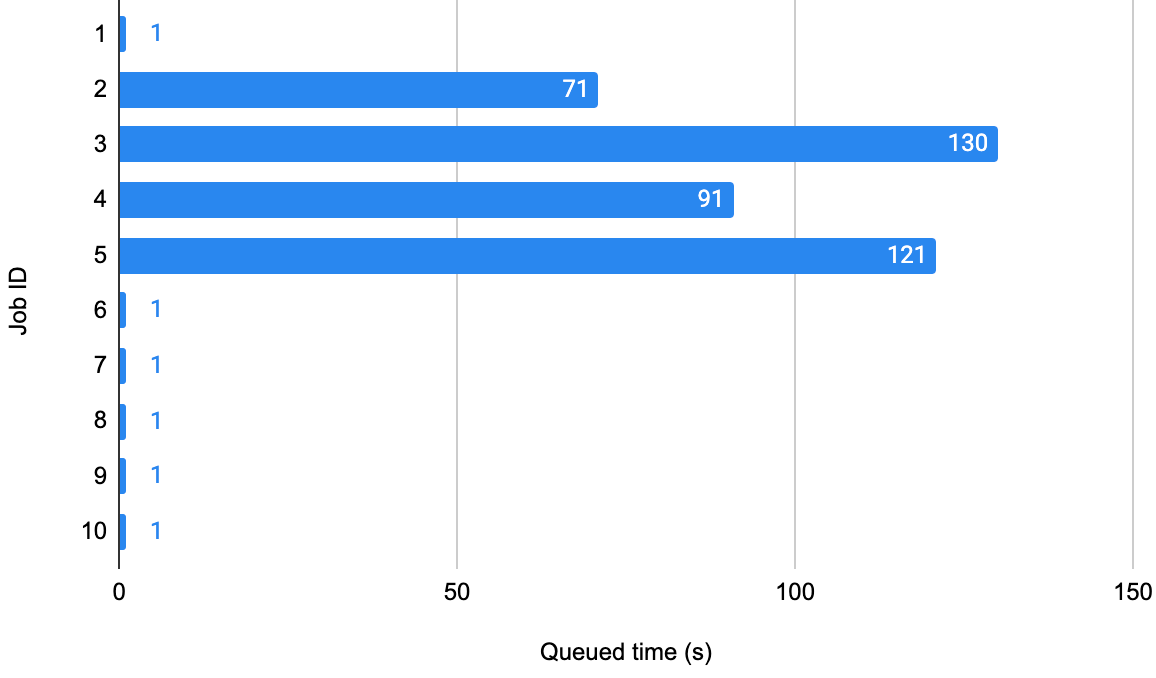
\includegraphics[width=0.90\textwidth]{pics/queued_time.png}
  \caption{Observation of Queued Time in AWS Integrated Toolchain During The runtime Experiment, When 10 Jobs Run in Parallel}
  \label{fig:queued}
\end{figure}
 \par
 The runtime of the non-integrated toolchain is also slightly going up because of the runtime of the build and push container to ECR increases. The reason is obvious, we have these two stages runs on the master node, so the increased data transfer between agent and master and limited computing resource on the Jenkins master increase the runtime. However, as we observed in Experiment 1, the build stage is always fully paralleled, and the runtime of this stage remains unchanged despite the increasing workload. The queuing time for resource in each job is negligible.
 \subsubsection{Cost Analysis}
 As a serverless tool, AWS DevOps tooling charges us according to the time and type of hardware configuration (in CodeBuild) we are using.
  Each pipeline in CodePipeline cost \$1 per month, which is a negligible amount of \$0.0014 per hour, price of with the build agent type general1.small (Linux instance with 3GB Memory and two vCPU) that we used in the experiment is \$0.3 per hour. The CodeDeploy is free of charge under the condition that we are not deploying to on-premises servers. The cost of S3 which store artifacts (less than 1 MB in our case) is negligible according to AWS\footnote{https://aws.amazon.com/getting-started/projects/set-up-ci-cd-pipeline/services-costs}. In conclusion, the price should be \$0.30014 per running job for one hour's runtime.
  \par
  In our non-integrated toolchain, our experiment setup (2 vCPU, 4 GB RAM) is different from what we have in 5.1. The price should be \$0.1029 per running agent for one hour's runtime. While the cost of EC2 instance that hosts the Jenkins master node costs \$0.0432 per hour, this price will remain constant when multiple jobs run in parallel. In general, the cost of the non-integrated toolchain is \$0.1452 per hour when only one agent is running.
From the calculation, we can see that the AWS integrated toolchain is more expensive under similar performance.
\subsection{Conclusion}
By analysing and explain the results, we could see that two toolchains have similar performance when it runs our case project. However, by further observe the runtime in each stage, we notice that the AWS integrated toolchain is faster in provisioning the build environment, but, slower in running the build and testing task itself. Such runtime distribution means it might be suitable for light but more frequent build task. 
The software project in real-life software development is much larger, and as a result, the build time will take a larger proportion in the total runtime. Therefore, the AWS integrated toolchain may become slower since it's building is slower than Jenkins non-integrated toolchain.
From the parallel execution part, we conclude that with our AWS integrated toolchain, the AWS CodeBuild, which takes most of the runtime, do have a limitation on the resource that we can use at the same time. Thus, before the system provisioning any resource, some tasks have to wait for the resource allocation in the "Queued" status. The "Queued" status largely prolongs the total runtime. 
\par
In general, the AWS integrated toolchain is more expensive and slower than our Jenkins-centred non-integrated toolchain, note that this does not mean the non-integrated is better than integrated toolchain. As we discussed in the last chapter, the AWS integrated toolchain is easier and faster to implement, is more stable and with better customer support. Table \ref{tab:exp2} summarised the result of this experiment.
\begin{table}[]
    \centering
    \begin{tabular}{|l|l|l|}
    \hline
     &
      \multicolumn{1}{c|}{\begin{tabular}[c]{@{}c@{}}Jenkins-centered \\ Non-integrated Toolchain\end{tabular}} &
      \multicolumn{1}{c|}{AWS Integrated Toolchain} \\ \hline
    Build Time &
      \begin{tabular}[c]{@{}l@{}}Slighter faster(123s), better \\ performance under parallel \\ build because Fargate \\ instances does not competing \\ for resources with each other.\end{tabular} &
      \begin{tabular}[c]{@{}l@{}}125s for a single task. \\ Increased with the number \\ of the parallel executing task \\ goes up, could be because \\ of the queueing for the\\ resources within CodeBuild.\end{tabular} \\ \hline
    Cost &
      \begin{tabular}[c]{@{}l@{}}Lower per hour price, \\ \$0.1452 per running \\ agent (includes the cost \\ of master node).\end{tabular} &
      \begin{tabular}[c]{@{}l@{}}Higher per hour price, \\ \$0.3 per hour per running \\ CodeBuild agent.\\ However no constant \\ additional cost as the master\\ node in Jenkins, might be \\ cheaper in a long run.\end{tabular} \\ \hline
    \end{tabular}
    \caption{Result of Experiment 2}
    \label{tab:exp2}
    \end{table}